\section{Mathematical Analysis}
\subsection{OpenCV algorithms}
    \subsubsection{Image representation}
      The core of the system would mainly deal with images. The structures which store images determine both the way the data is wrapped but also the approach for algorithms to take. All images are composed of pixels. An image is a matrix of them. In OpenCV, images can be of different color spaces. Different color spaces might require different number of channels (thus different amount of memory) to describe one pixel. The most important in this project are \verb|BGR| and \verb|GRAY| color spaces. \verb|BGR|, which is the default color format in OpenCV is often referred as RGB, but in OpenCV the order of bytes is reversed. \verb|GRAY| is a color space described by one channel which represents the intensity of the pixel, basically describing the transition from white to black. Thus each pixel is a set of numerical values, indicating the intensity of the corresponding channel. Using this representation, images can be added, subtracted or multiplied, between them or by a constant. All these operations are performed on matrices which stand behind the images. 
    \subsubsection{OpenCV built-in algorithms}

      As OpenCV is mostly a library of different algorithms, the following section describes OpenCV methods which were used in this thesis. As mentioned in the previous chapter, the first task is to identify the objects. This leads to the necessity of shadow elimination and background subtraction. Both of these algorithms are implemented in \verb|BackgroundSubtractorMOG2| class from OpenCV. The class implements the updated Gaussian mixture model background subtraction described in ``Gaussian mixture model and Density Estimation for background subtraction'', \cite{zivkovic},  \cite{heijden}. The code is very fast and performs also shadow detection. The shadow is detected if the pixel is a darker version of the background. A threshold defines how much darker the shadow can be, \cite{prati}. Basically, this algorithm is used to determine the background from a video, where many frames are present. It works, though, with only two frames as well: the first frame represents the clear background and the second depicts the objects. In the way this algorithm works, it is very similar to the direct subtraction of these two images: the same pixels would have similar numerical values and their subtraction would result in zero -- giving a black color for the mask. Other pixels, where objects appeared, would have the numerical value different from zero; using a specific threshold they can be recolored to white color, thus resulting into a corresponding mask.

      \begin{figure}[t]
        \centering
        \subfloat[ Background image]
         {
         \label{background}
          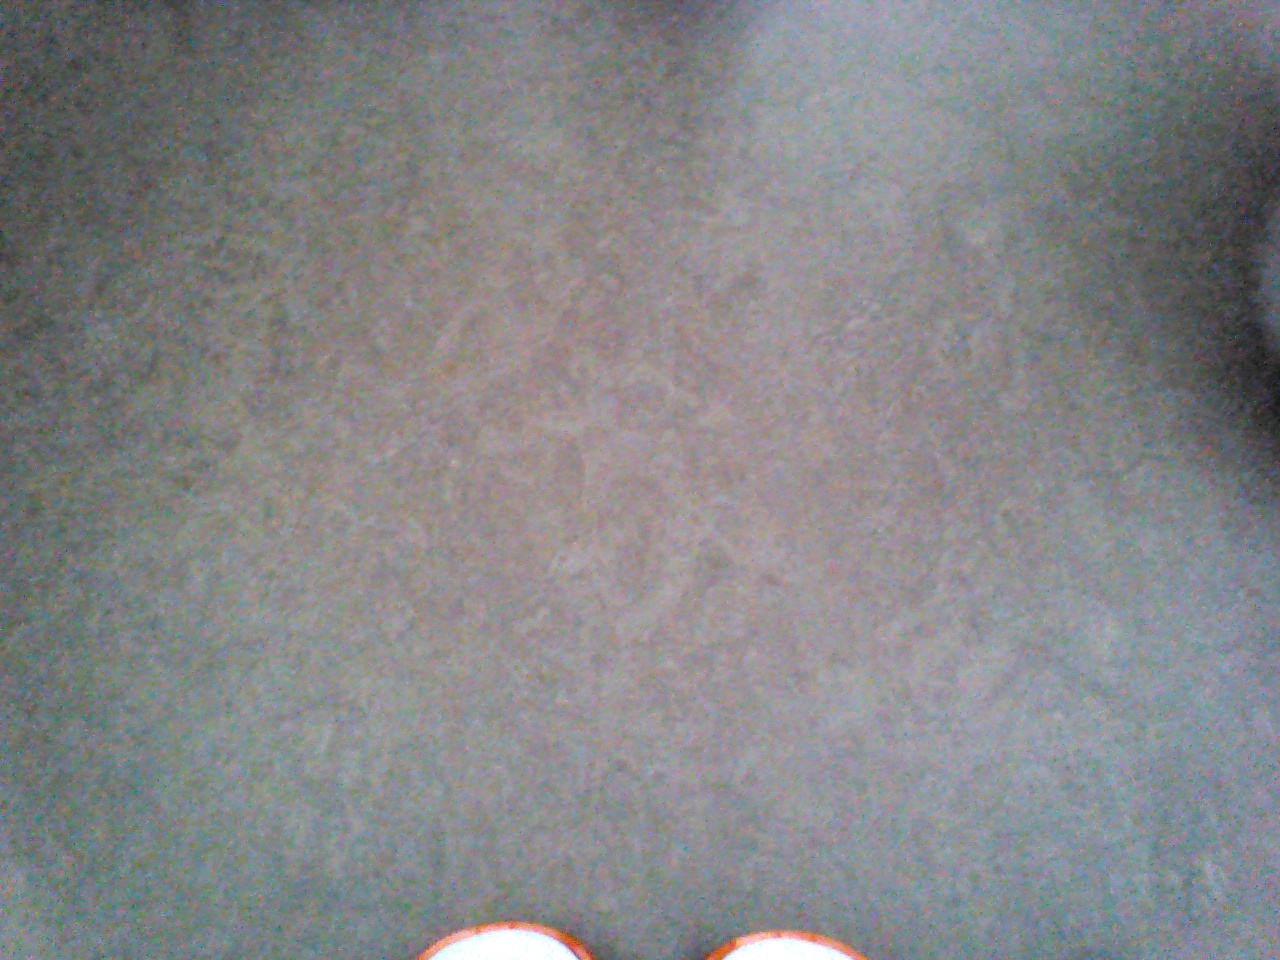
\includegraphics[width=0.45\linewidth]{7-1.jpg}
         }
        \hfil 
        \subfloat[ Image with objects]
         {
          \label{objects}
          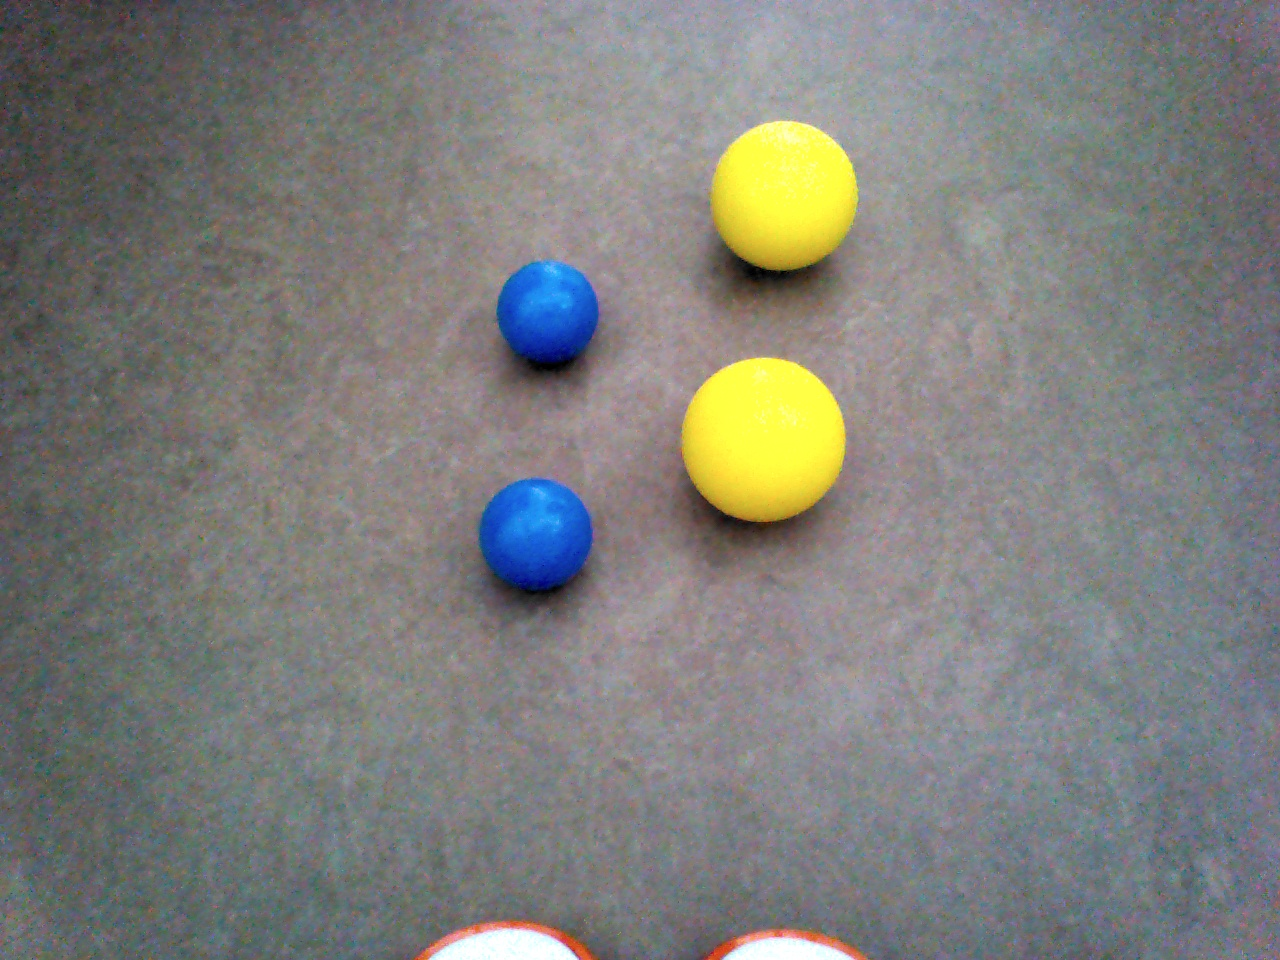
\includegraphics[width=0.45\linewidth]{7-2.jpg} 
         }
        \caption{Initial images}
        \label{backgroundAndObjects}
      \end{figure}

      As depicted in figure \ref{backgroundAndObjects}, there are two images. Remark the fact that in the background image (left one), at the right limit of the image there is a black spot, which disappears in the next image. This would affect the subtraction in figure \ref{mask}.
      \begin{figure}[t]
        \centering
        \subfloat[ Mask with shadow]
         {
         \label{withShadow}
          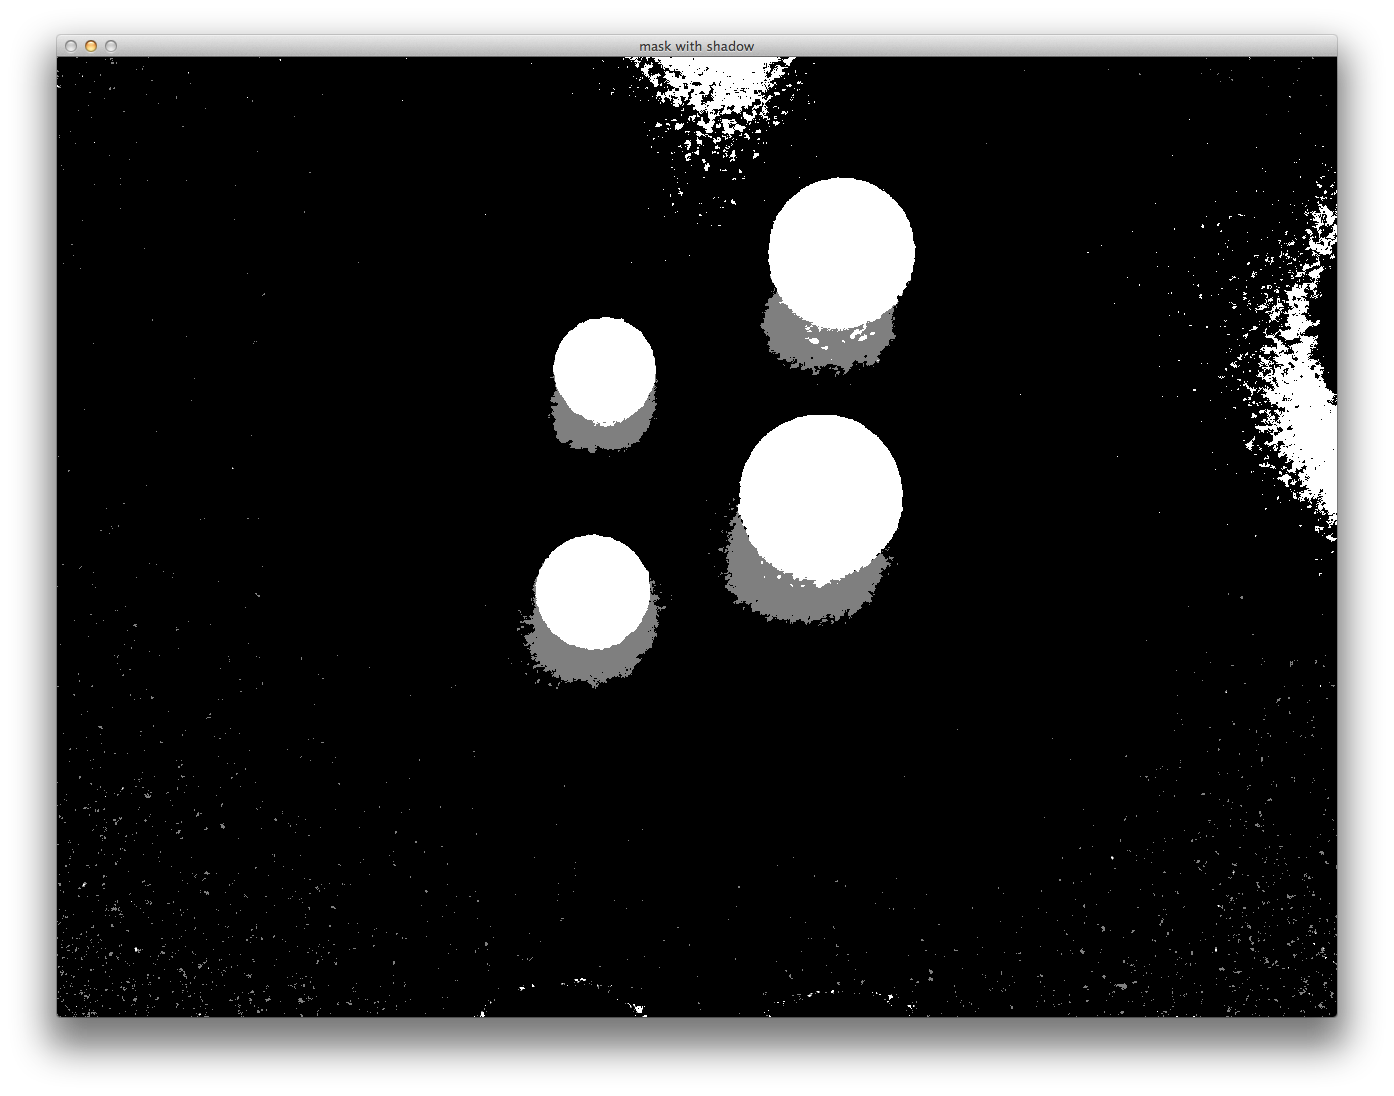
\includegraphics[width=0.45\linewidth]{8-1.png}
         }
        \hfil 
        \subfloat[ Mask without shadow]
         {
          \label{withoutShadow}
          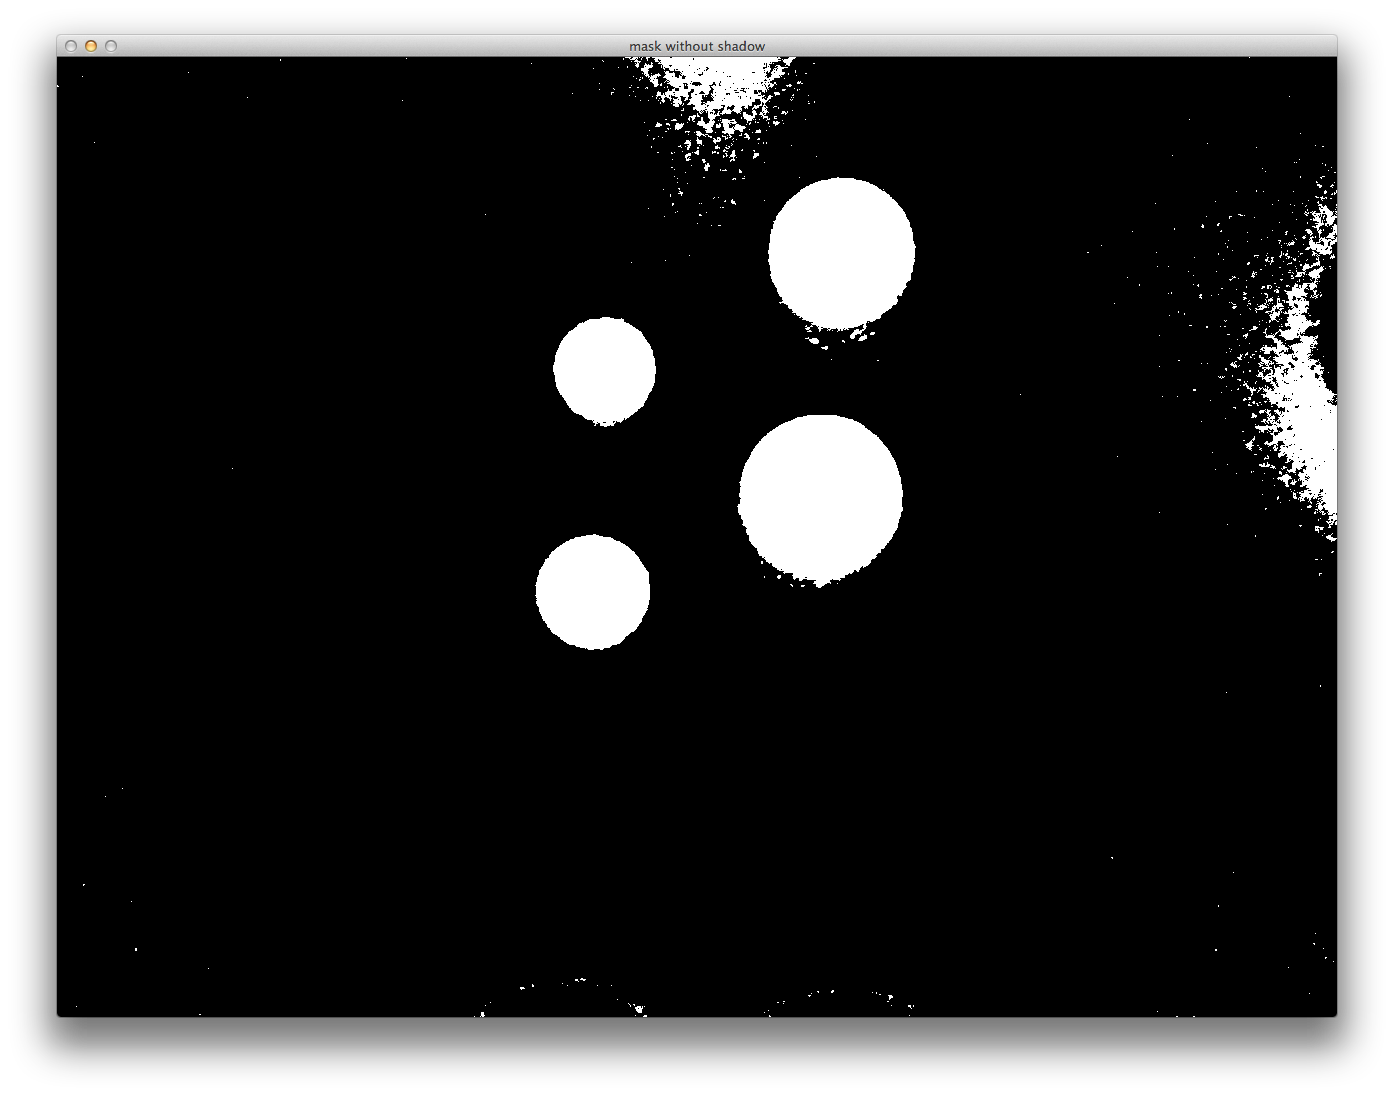
\includegraphics[width=0.45\linewidth]{8-2.png} 
         }
        \caption{Obtained mask after image processing}
        \label{mask}
      \end{figure}
Another interesting function used from OpenCV is the color space conversion. More precisely, there was a need for conversion from \verb|BGR| to \verb|GRAY| color space. \verb|BGR| has three channels while \verb|GRAY| has only one channel. The formula for this transformation, as presented in OpenCV documentation, \cite{opencv}, is:
\begin{equation}
        \label{conv}
          Y = 0.299\cdot R + 0.587\cdot G + 0.114\cdot B.
\end{equation}
      There are also other colorspace conversions which are not in the scope of this thesis. Smoothing or blurring is simple and frequently used image processing operation. To perform a smoothing operation a filter is applied over the image. The most common type of filters are linear, in which an output pixel’s value \(g(i,j)\) is determined as a weighted sum of input pixel values \(f(i+k,j+l)\):
\begin{equation}
        \label{wightedSum}
          g(i,j) = \sum_{k,l} f(i+k,j+l)h(k,l),
\end{equation}
      where \(h(k,l)\) is the so-called the kernel, which is nothing more than the coefficients of the filter. The utilized function smoothes an image using the following kernel: 
        \begin{eqnarray}
                \label{kernel}
          K = \frac{1}{k_{w}\cdot k_{h}} 
          \begin{bmatrix}
             1 & 1 & \cdots & 1 \\
             1 & 1 & \cdots & 1 \\
             \vdots  & \vdots  & \ddots & \vdots  \\
             1 & 1 & \cdots & 1 \\
           \end{bmatrix},
        \end{eqnarray}
where \( k_{w} \) is the kernel size width and \( k_{h} \) is the kernel size height.
      The most important in object detection are the functions for edge detection and creation of contours around the objects. These contours can be later enclosed in some rectangles, which can be cut from the initial image. Having as an input image the one as in the last figure, a threshold is specified which would depict the transition from black to white or vice-versa. The idea is based on a neighbor-pixels comparison. There are different approaches how to apply the threshold. For example, \verb|THRESH_BINARY| works in the following manner:
      \begin{equation}
       D(x,y) = \left\{ 
        \begin
          {array}{l l}
            V_{max} & \quad \text{if \(S(x,y)) > \nu_{T}\)}\\
            0 & \quad \text{otherwise},
        \end{array} 
        \right.
        \end{equation}
        where \( D \) is the destination matrix and \( S \) is the source matrix. \( V_{max}\) is the maximal value and \( \nu_{T}\) is the threshold. 
      Finally, in the obtained binary image the contours are found. The algorithm used in this function is presented in ``Topological Analysis of Binary Images'', \cite{suzuki}. The results of the images obtained in the last step would be as depicted in figure \ref{contours}.

      \begin{figure}[ht!]
        \centering
        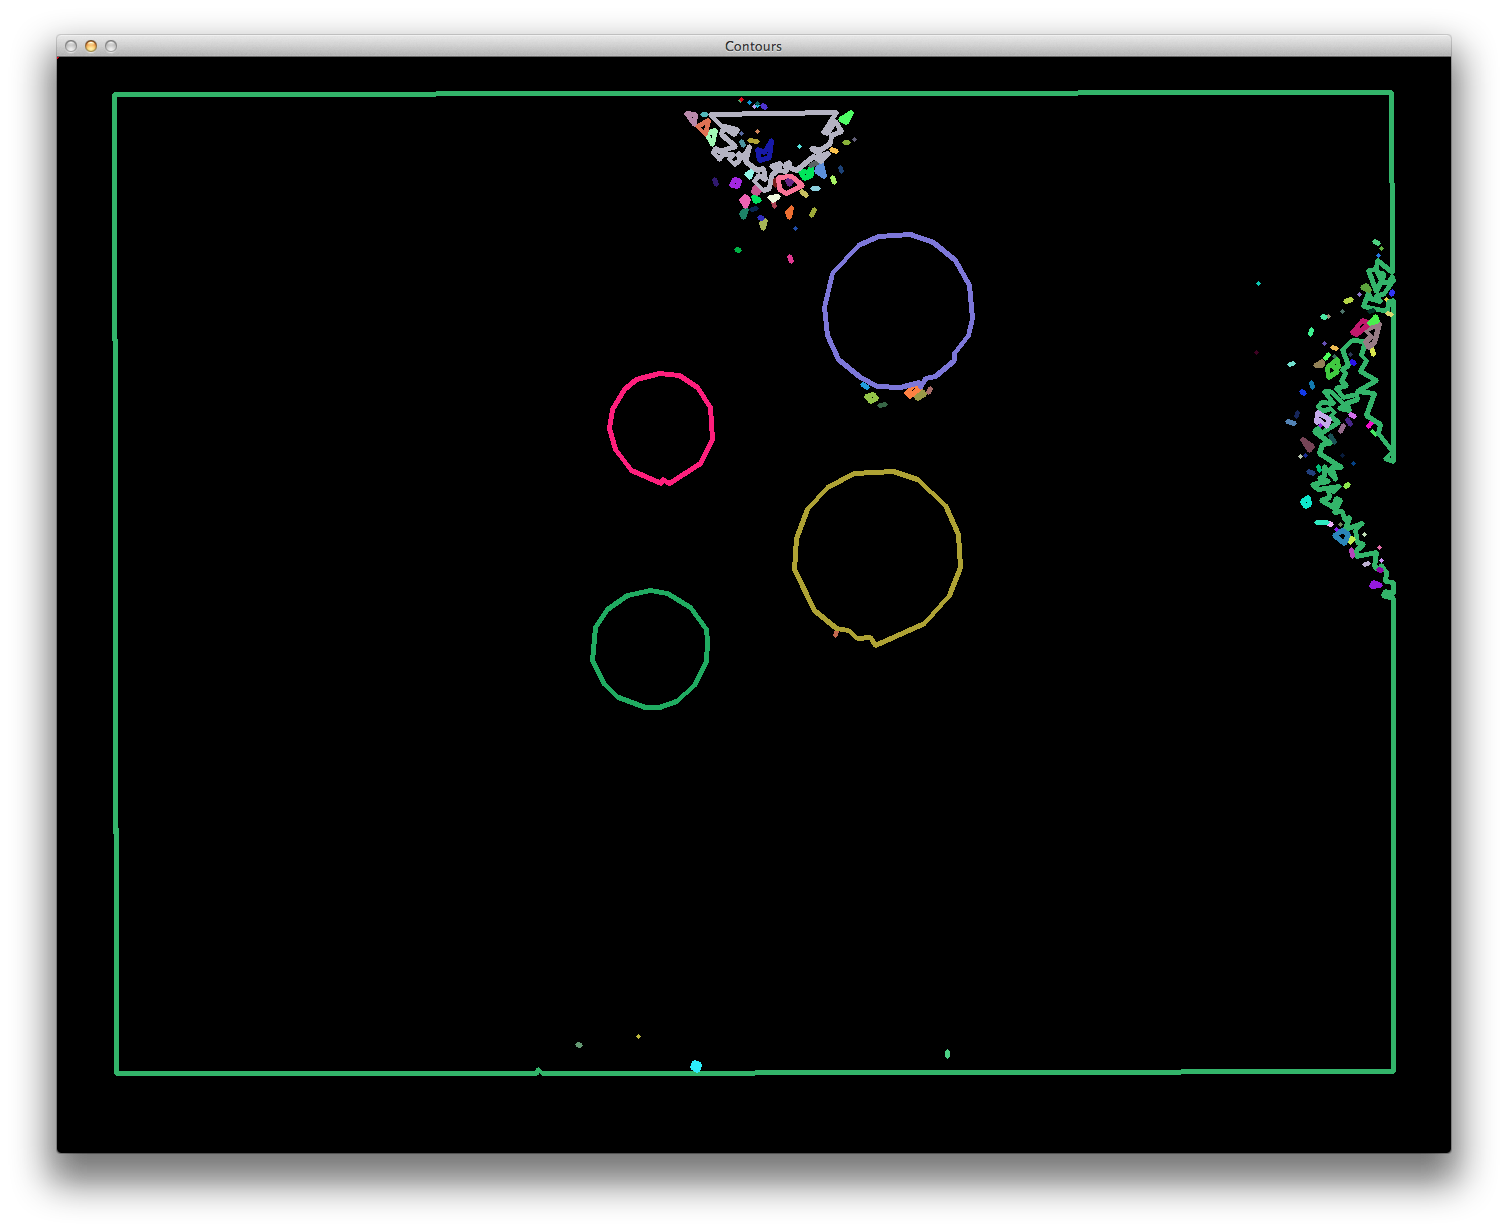
\includegraphics[width=0.8\linewidth]{9.png} 
        \caption{Contours of the detected objects and noise}
        \label{contours}
      \end{figure}

      As it is seen from the picture, there are multiple small contours which resulted because of the noise. Latter an easy way to tackle this problem will be presented. But before enclosing these figures into rectangles, a function for polygon approximation is used. This function approximates a curve or polygon with another curve/polygon with less vertices so that the distance between them is less or equal to the specified precision. It uses the Ramer-Douglas-Peucker algorithm. The simplified curve consists of a subset of the points that defined the original curve. The simplified idea would be to remove the points which are closer to the current line than some epsilon distance (initially the current line is the line formed by the first and last point). Finally, the program computes the bounding rect for each contour. As mentioned earlier, there are a lot of small contours which are useless in terms of objects the system needs to detect. It is easy to eliminate them by setting a lower bound for area the rectangle needs to have. In a similar fashion the very big rectangle which covers almost all picture is eliminated, by adding a upper bound on area. As a result the following rectangles are returned:

      \begin{figure}[t!]
        \centering
        \subfloat[ On the model image]
         {
         \label{black}
          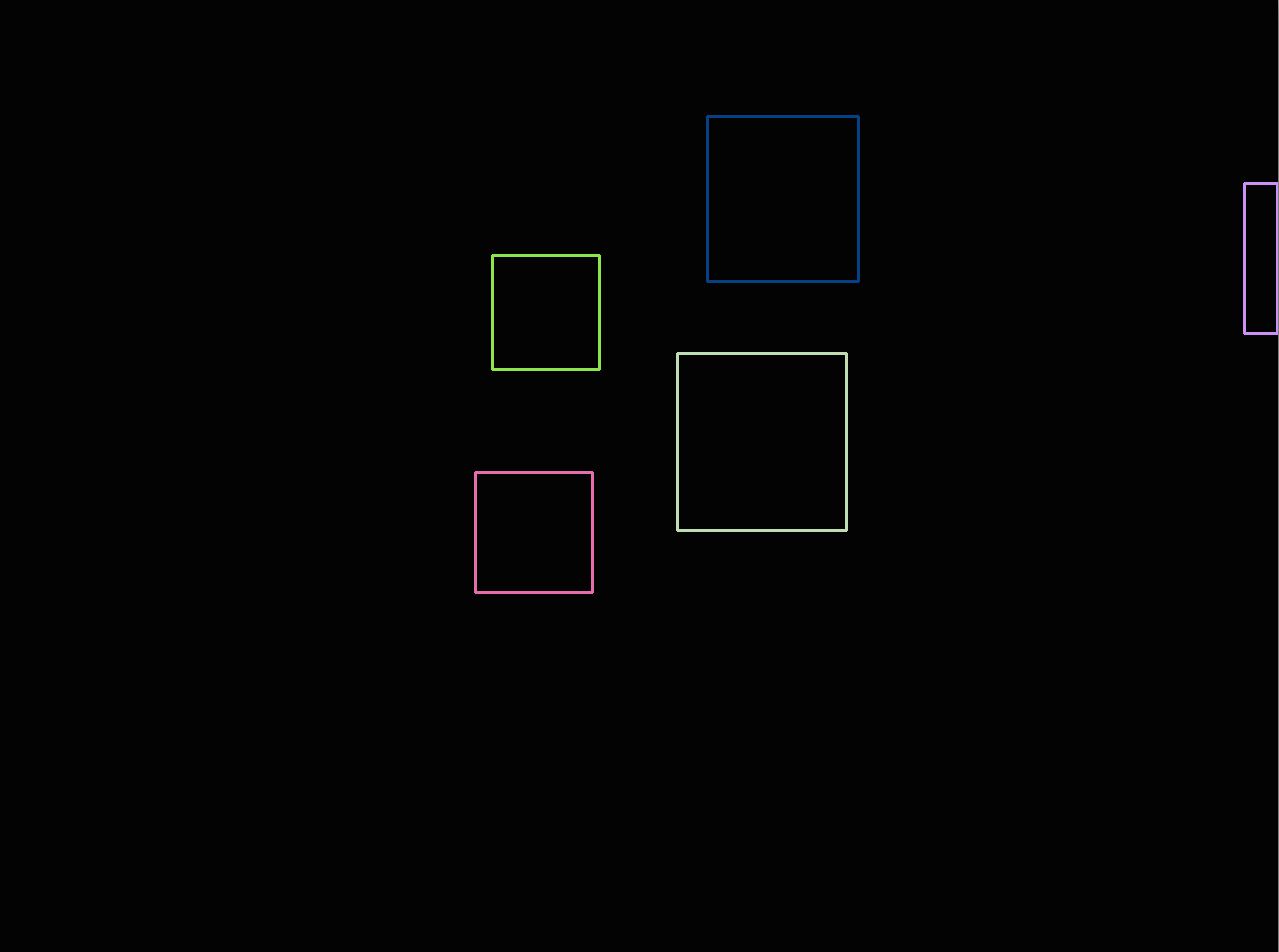
\includegraphics[width=0.45\linewidth]{10-1.png}
         }
        \hfil 
        \subfloat[ On the original image]
         {
          \label{onImage}
          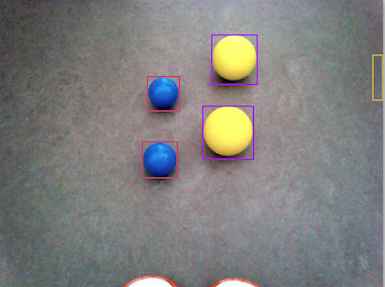
\includegraphics[width=0.45\linewidth]{10-2.png} 
         }
        \caption{Detected objects are enclosed into rectangles}
        \label{rectangles}
      \end{figure}

      Finally, the last algorithm from OpenCV which is used in this project is K-Means clustering algorithm. A more detailed description of it would follow in Machine Learning algorithms section. At first, a custom implementation of it was used. Later, for comparison reasons, the one implemented in OpenCV was added. While both perform quite well, the one from library gives a slightly better result and is optimized. The disadvantage of it was the fact that it does not determine by itself the number of clusters, thus a combination of OpenCV implementation of K-means together with custom determination of the number of clusters was used. 

The algorithm from library finds the centers of \( n\) clusters (where \( n\) is given) and groups input samples around the clusters. As an output an array of labels is returned, where element \( i\) contains a 0-based index for the sample stored in the \(i\)-th row of the matrix of samples. The function returns the compactness measure that is computed after every attempt:
        \begin{equation}
        \label{sumsum}
          \sum_{i} \| S_{i} - C_{L_{i}} \|^{2},
        \end{equation}
      where \( S_{i}\) is the vector of samples of \( i \) and \( C_{L_{i}} \) is the vector of centers which have the labels \(L_{i} \). The best (minimum) value is chosen and the corresponding labels and the compactness value are returned by the function, \cite{opencv}.


    \subsection{Distance computation}

      NAO has to reach and grasp the objects. In order to achieve that, he needs to know the location of the objects in space. The information which he has is the location of objects in the image and the position of the camera. Given that, it is possible to determine the distance between camera and objects. NAO's current position in space is also known. Concluding, the available information is enough to compute both the position of objects in space and the distance between them and NAO. 
      % In order to solve this problem, a selection of a coordinate system is needed.

      \subsubsection{NAO coordinate systems}

        NAO deals with three coordinate frames. For This project, two of them are important. The first one, denoted as \verb|FRAME_ROBOT|, has the origin in the average of the two feet positions projected around a vertical \(z\) axis. This space is useful, because the \(x\) axis is always forward, so provides a natural ego-centric reference. The second one is \verb|FRAME_WORLD|, which is a fixed origin that is never altered. It is left behind when NAO walks, and will be different in \(z\) rotation after NAO has turned. This space is useful for calculations which require an external, absolute frame of reference, \cite{naoDocumentation}. The figure \ref{axis} depicts how the axes in all coordinate spaces are oriented. 

        \begin{figure}[ht!]
        \centering
        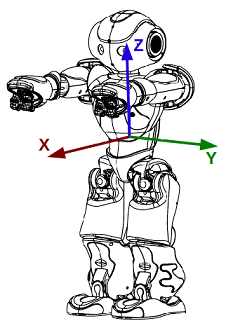
\includegraphics[width=4cm]{13.png} 
        \caption{Axes definition of the NAO's TORSO FRAME coordinate system, \cite{naoDocumentation}}
        \label{axis}
        \end{figure}

      An object in the image is bounded by a rectangle. Its position in image can be approximated to the center of that rectangle. The coordinates in the picture start in the top-left corner, \(x\) growing to the right, and \(y\) growing to the bottom of the image. 
A camera has horizontal and a vertical angle of view. The horizontal angle of view limits the distance to the left and right the camera can catch and the vertical angle of view limits the distance in the up and down directions which camera can catch. Translated to the NAO's coordinate systems axes, the vertical angle defines how far NAO can see on the NAO's \(x\) axis, horizontal angle -- on NAO's \(y\) axis. 
      If an object is higher in the image that means it is farther away in the forward direction. If an object is closer to the left side of the image, it should have a bigger value on the \(y\) coordinate of NAO's frame. 

      \begin{figure}[b!]
        \centering
        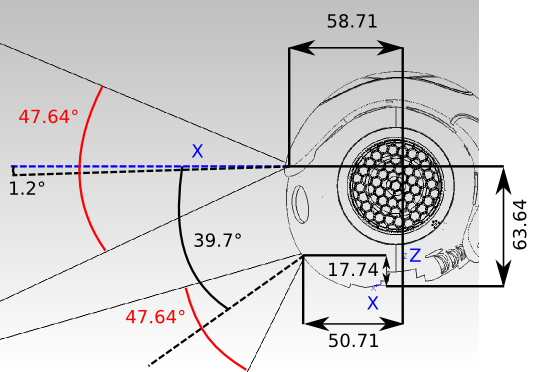
\includegraphics[width=0.75\linewidth]{14.png} 
        \caption{Angles and ranges of view of NAO's cameras, \cite{naoDocumentation}}
        \label{angles}
      \end{figure}

      NAO's camera position is available. The objects are located in the area close to NAO, so the bottom camera is used. This camera has a bigger angle of inclination with the NAO's \(x\) axe so that it ``looks down''. So this camera is used exclusively for all image acquisition. The position of the camera is described in \(x, y, z, wx, wy, wz\), where \(wx, wy, wz\) are the rotations around the corresponding axes. Thus the height of the camera and its inclination around \(y\) axis is available. Using simple Pythagorean theorem it can be computed how far the camera ``can see'' in the forward direction. But a camera has a vertical range of view, that is an angle of view which camera can percept. The current computed forward distance corresponds to the middle of this range of view. The lowest point in the image would correspond just to the start of the range of view, while the highest point -- to the end of it. Having the vertical angle at which the object lays it is possible to compute the forward distance toward it. The vertical range, as depicted in figure \ref{angles}, is \(47.64\) degrees.

      \subsubsection{Forward distance computation}

        The following formulas show how the object position is computed:
        \begin{equation}
          Y = \frac{N_{y} - O_{y}}{N_{y}},  0 < Y \leq 1,
        \end{equation}
        where \(Y\) represents the percentage of object's \(y\) coordinate in the image, \( N_{y}\) is \( y\) coordinate of NAO's position of the image and \( O_{y}\) is object's \( y\) coordinate in the image. If \(Y = 0\), it means the object is right at the bottom of the image; if \(Y = 1\), it means the object is right at the top of the image. \(N\) point is the position of NAO if he would be on the image. It was computed by solving the opposite problem to one which is explained now, but since there were more unknowns than equations, a heuristic approach was used. Basically, this position was approximated until the result was good enough. This position is a fixed position on the image before starting movement. The image has the size of \((1280,960) px\). NAO start position is \((640, 1070.43) px\). The position of the objects is calculated only once, before any movement. Next, the actual angle is computed (it is notated by \(\beta\)), which would be used to determine the forward distance. Angle \(\beta\) is the angle between the hypotenuse and the height of the camera and the remaining cathetus is the unknown forward distance.
        \begin{equation}
          \beta = 90 - \alpha - \frac{\gamma_{1}}{2} + Y\cdot \gamma_{1},
        \end{equation}
        where the \(\alpha\) is the angle of rotation of the camera around \(y\) axis retrieved from sensors before computation and \( \gamma_{1}\) denotes the range of vertical view. Finally, the forward distance \(F\) is:
        \begin{equation}
          F = h\cdot \tan \beta,
        \end{equation}
        where \(h\) is the camera height.

      \subsubsection{Lateral distance computation}
        Computing lateral distance, there is a need to take into acount the fact that farther is the point on the image, wider is the lateral distance. The horizontal range of view is increasing the distance on \(x\) axis as the look goes farther forward, as depicted in figure \ref{horizontalRange}.
        
        \begin{figure}[b!]
          \centering
          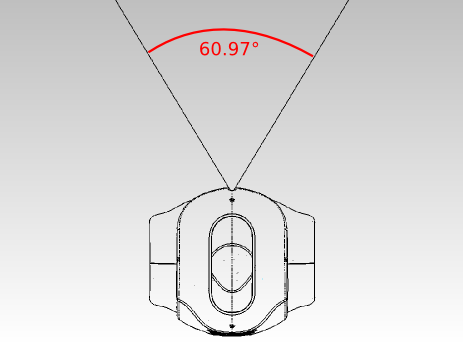
\includegraphics[width=0.6\linewidth]{15.png} 
          \caption{NAO's camera horizontal range of view, \cite{naoDocumentation}}
          \label{horizontalRange}
        \end{figure}

        In a similar way to \(Y\) coordinate, the \(X\) coordinate is expressed: 
        \begin{equation}
          X = \frac{O_{x} - \frac{I_{w}}{2} + N_{x}}{I_{w}},
        \end{equation}
          where \( I_{w}\) is the image width. If \(X = 0\) the object is on the left limit of the image; if \(X = 1\) the object is on the right limit of the image. Now, there are a two right triangles to deal with. The first one was already described -- it is the triangle formed by \(h\), \(F\) and \(\beta\) angle. Let's denote the hypotenuse of this triangle as \(P\). \(P\) represents the camera projection distance. The second triangle is formed by \(P\), \(L\) (lateral distance) and the angle \(\theta\), which is possible to compute. To compute distance \(P\) Pythagorean theorem is applied again:
          \begin{equation}
            P = \sqrt{F^2 + h^2}. 
          \end{equation}
           To compute angle \(\theta\) first angle \( \omega \) is calculated:
          \begin{equation}
        \omega = \frac{\gamma_{2}}{2},
          \end{equation}
          where \( \omega \) is the width angle and \(\gamma_{2}\) denotes the range of horizontal view. The angle \( \theta \) is:
          \begin{equation}
                \theta = -\omega + X\cdot \gamma_{2}.
          \end{equation}
          So the lateral distance would be:
          \begin{equation}
            L = h\cdot \tan \theta.
          \end{equation}
              Finally, to compute the object position, the above-calculated distances are added to the robot's current position. To verify how precise these results are, a series of tests were run. The image was divided into 12 zones and objects were placed in these zones. Their actual and computed positions were stored, then the error was computed. The results of measurements are presented in the table \ref{tab:items}. 
\begin{table}[t!]
\centering
\caption{Distance computation precision by NAO}
{
\renewcommand{\arraystretch}{2}
\begin{tabular}{ c|c|c|c|c|c|c }
\hline           
 Nr & \pbox{4cm}{Forward \\distance, m} &\pbox{5cm}{Lateral \\distance, m} &  \pbox{7cm}{Forward \\error, m} & \pbox{7cm}{Lateral \\error, m} &
  \pbox{7cm}{Forward \\error, \%} & \pbox{7cm}{Lateral \\error, \%} \\ \hline \hline
          1 & \( 0.4664 \) & \( -0.2181 \) & \( -0.0143 \) & \( 0.0357 \) & \( 1.2477 \) & \( 16.3769 \) \\ 
          2 & \( 0.4241 \) & \( -0.0500 \) & \( -0.0080 \) & \( 0.0046 \) & \( 0.6159 \) & \( 9.1024 \)  \\ 
          3 & \( 0.4241 \) & \( 0.1000 \) & \( -0.0026 \) & \( -0.0031 \) & \( 0.0760 \) & \( 3.0779 \) \\ 
          4 & \( 0.4509 \) & \( 0.2296 \) & \( -0.0206 \) & \( -0.0513 \) & \( 1.8835 \) & \( 22.3358 \) \\ 
          5 & \( 0.3000 \) & \( -0.1500 \) & \( 0.0054 \) & \( 0.0200 \) & \( 0.7200 \) & \( 13.3333 \) \\ 
          6 & \( 0.3500 \) & \( -0.0500 \) & \( 0.0019 \) & \( 0.0091 \) & \( 0.3728 \) & \( 18.2876 \) \\ 
          7 & \( 0.2900 \) & \( 0.0400 \) & \( 0.0032 \) & \( 0.0029 \) & \( 0.5032 \) & \( 7.2840 \) \\ 
          8 & \( 0.3100 \) & \( 0.1800 \) & \( 0.0009 \) & \( -0.0176 \) & \( 0.2693 \) & \( 9.7889 \) \\ 
          9 & \( 0.2500 \) & \( -0.1518 \) & \( 0.0034 \) & \( 0.0179 \) & \( 0.5200 \) & \( 11.7958 \) \\ 
          10 & \( 0.2400 \) & \( -0.0500 \) & \( 0.0063 \) & \( 0.0082 \) & \( 0.8072 \) & \( 16.4072 \) \\ 
          11 & \( 0.2300 \) & \( 0.0300 \) & \( 0.0034 \) & \( -0.0028 \) & \( 0.5216 \) & \( 9.2617 \) \\ 
          12 & \( 0.2400 \) & \( 0.1500 \) & \( -0.0011 \) & \( -0.0240 \) & \( 0.0711 \) & \( 15.9953 \) \\ \hline
          Mean & \( - \)  & \( - \) & \( 0.0060 \) & \( 0.0164 \) & \( 0.6340 \) & \( 12.7539 \) \\ \hline 
\end{tabular}
}
\label{tab:items}
\end{table}
      The forward distance computation is accurate enough. The average forward error is 0.6cm. The maximal forward error is almost 2cm. The lateral error, on the other hand, is bigger. Its mean error is 1.6cm. The maximal lateral error is almost 5cm. The forward and lateral distances themselves are quite small, bounded at 47cm and 23cm respectively. An error of 2-3cm is still acceptable in order for NAO to reach the destination and in the end grasp the object.


  \subsection{Machine learning algorithms}
    \subsubsection{K-means clustering}
          The materials presented in this section are integrally based on Machine Learning online course, \cite{ml}. Some of figures and formulas are taken from slides of this course, \cite{slides}.
Given a set of points, clustering is labeling each point with the group it belongs to. If all the points are similar, there might be just one cluster (group). In Machine Learning, the input points are denoted as \textbf{training set}. Clustering is used in Market segmentation, Social network analysis, Logistic of computer clusters and Astronomical data analysis, \cite{slides}. Mathematically, a training set is a vector of points:
      \begin{equation}
        [ x^{(1)}, x^{(2)}, \cdots, x^{(m)} ],
      \end{equation}
      where \( x^{(i)}\) denotes the training example \(i\). As a result, clustering should give a vector of labels:
      \begin{equation}
        [ y^{(1)}, y^{(2)}, \cdots, y^{(m)} ],
      \end{equation}
      where \( y^{(i)}\) represents the label for the training example \(i\). K-means algorithm itself takes the following input:
      \begin{gather}
        \nonumber
            K - \text{number of clusters} \\
            \nonumber
            [ x^{(1)}, x^{(2)}, \cdots, x^{(m)} ] - \text{training set} \\
            \nonumber
            x^{(i)} \in \mathbb{R}^n
      \end{gather}
      The \emph{K-Means algorithm} is presented below:
      \begin{algorithm}
        {Randomly initialize \(K\) cluster centroids $\mu_1, \mu_2, \cdots, \mu_K \in \mathbb{R}^n$}
        \begin{algorithmic}
          \Repeat 
          % \State {\emph{Cluster assignment step:}}
            \For{\( 1 \leq i \leq m \)}
              \State {\( c^{(i)} = \) index (from 1 to K) of cluster centroid closer to \( x^{(i)} \)} 
            \EndFor
          % \State {\emph{Centroid movement step:}}
            \For{\( 1 \leq k \leq K \)}
              \State {\( \mu_{k} = \) average (mean) of points assigned to cluster \( k \)} 
            \EndFor
          \Until{no changes}
        \end{algorithmic}
        \caption{K-Means algorithm}\label{alg:kmeans}
      \end{algorithm}
      \newline
      This algorithm consists of two steps. Each step is represented by a loop. The first \verb|for| loop is the \emph{Cluster assignment step}. In this step each point is assigned a label. This label represents the cluster which is the closest to the given point. The second step is represented by the second \verb|for| loop. This step is called \emph{Centroid movement step}. After the first step, each centroid has a number of points assigned to it. It recalculates the new position of the center (centroid) by computing the geometrical center of all the points. The process repeats until convergence -- the step after which label of points and the positions of centroids are unchanged.
        In figure \ref{pointsAndClusters} the result of a clustering is shown. 
              \begin{figure}[h!]
        \centering
        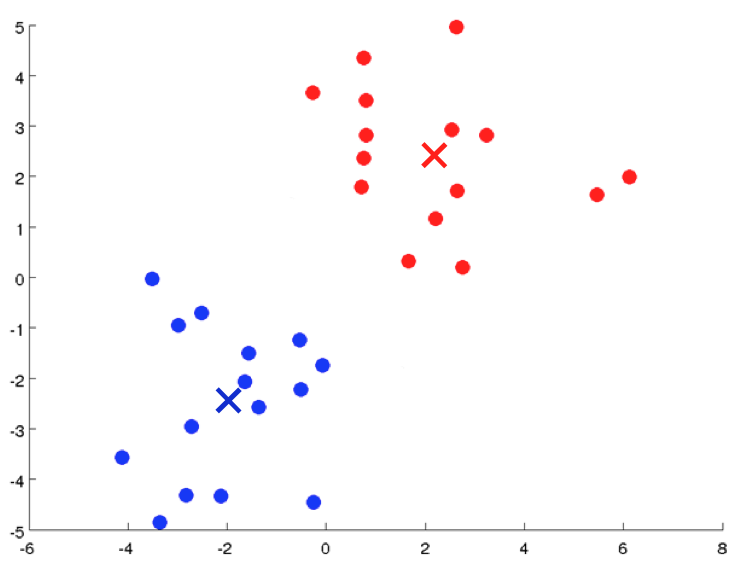
\includegraphics[width=0.45\linewidth]{16.png} 
        \caption{Points clustered into two clusters by K-means algorithm, \cite{slides}}
        \label{pointsAndClusters}
      \end{figure}

        \noindent The dots represent the points of the training set and the crosses are the centroids. The color shows the label of each point.
        In the start of the algorithm a random choice of centroids is performed. A different choice of centroids might lead to different results. This is usually not the desired result. In order to obtain the best result, the algorithm is run multiple times and the best outcome is chosen. The best outcome is the one which has the smallest error. A definition of the error function is needed. Given the following definitions:
        \begin{gather}
        \nonumber
          c^{(i)} - \text{index of cluster } (1, 2, ... , K) \text{ to which example } x^{(i)} \text{ is currently assigned}; \\
          \nonumber
          \mu_k - \text{cluster centroid } k  \text{ } (\mu_k \in \mathbb{R}^n); \\
          \nonumber
          \mu_{c^{(i)}} - \text{cluster centroid of cluster to which example } x^{(i)} \text{ has been assigned}.
        \end{gather}
        The error function is:
        \begin{equation}
          J(c^{(1)}, ..., c^{(m)}, \mu_1, ..., \mu_K) = \frac{1}{m}\sum_{i=1}^{m}\|x^{(i)} - \mu_{c^{(i)}}\|^2
        \end{equation}
        Basically the error function says that the error of clustering is the average of errors of each point, where the error of one point is the Euclidean distance between point and centroid. Having the error function, it is possible to define the optimization objective:
        \begin{equation}
        \begin{aligned}
        & \underset{ \mu_1, ..., \mu_K} { \underset{c^{(1)}, ..., c^{(m)}} {\text{min}} }
        & &  J(c^{(1)}, ..., c^{(m)}, \mu_1, ..., \mu_K)
        \end{aligned}
        \end{equation}
        Thus the goal is to minimize the error function. At the start of the algorithm a random initialization is performed. Random initialization consists of the following steps:
        \begin{enumerate}[topsep=5pt, partopsep=0pt,itemsep=3pt,parsep=1pt]
        \item Assure that \( K < m \) (number of clusters is less than the number of training examples);
        \item Randomly pick \( K \) training examples;
        \item Set \( \mu_1, ..., \mu_K \) equal to these \( K \) examples.
        \end{enumerate}


        Multiple runs of the algorithm are important because as previously mentioned, different choices of centroids lead to different results. This might happen because of local optimas of the optimization functions. In figure \ref{localOptimas} an example is shown how algorithm converged to the local optima. Thus the complete version of algorithm is presented in algorithm \ref{alg2}. In Machine Learning, the error function is usually called the \textbf{cost function}.
                \begin{figure}[h!]
          \centering
          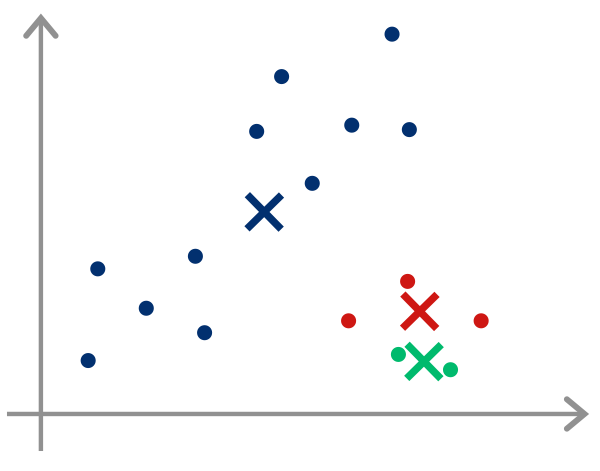
\includegraphics[width=5cm]{17.png} 
          \caption{Local optimas, \cite{slides}}
          \label{localOptimas}
        \end{figure}

      A custom implementation of K-means was done. Later it was compared with OpenCV built-in implementation. The second one was proven to be better, giving a smaller error. But the custom implementation could determine automatically the needed number of clusters. The technique used to determine the ``good'' number of clusters is called ``Elbow method''. In the end, the OpenCV implementation together with ``Elbow method'' were used:

        \begin{algorithm}
          \begin{algorithmic}
            \For{\( 1 \leq i \leq 100 \)} {\\}
              {Randomly initialize K-means \\}
              {Run K-means. Get \( c^{(1)}, ..., c^{(m)}, \mu_1, ..., \mu_K \).  \\}
              {Compute cost function(distortion) \( J(c^{(1)}, ..., c^{(m)}, \mu_1, ..., \mu_K) \).}
            \EndFor
            {Pick clustering that gave lowest cost \( J(c^{(1)}, ..., c^{(m)}, \mu_1, ..., \mu_K) \)}
        \end{algorithmic}
        \caption{K-Means algorithm with multiple runs}\label{alg2}
      \end{algorithm}



    \subsubsection{Elbow method}

      It is important to choose the right number of clusters -- \( K \). Sometimes even humans have different perspectives -- how would they group some objects -- it depends of their way of thinking. The desired effect is that when humans clearly see 4 different groups, so should the algorithm determine that there are 4 clusters. This number, \( K \), varies from 1 to \( m \), where \( m \) is the number of training examples. Indeed, there are two extremes: either all points go into one group, either each point is ``unique'', thus it cannot be grouped with others. The Elbow method offers a suggestion how this dilemma can be tackled. The idea is to look at the error. Given that the error is expressed in the distance of a point from the cluster, it is clear that if there are as many clusters as points, the error is zero -- each point is a cluster and each point is located in the same position as the centroid, distance being zero. So as the number of clusters increases, the error goes down. The interesting thing is that while the number of cluster increases and there are indeed enough groups for such a number, the error decreases very fast. As soon as \( K \) hits the optimal number, the error decreases at a slower speed. In figure \ref{elbow} a dependence of error to \( K \) is presented. As depicted, in the moment when \( K \) is optimal and the desired number of groups is hit, the slope of the line significantly changes, creating what is called ``the elbow'' (while the whole graph should be compared to an arm). 

      \begin{figure}[b!]
        \centering
        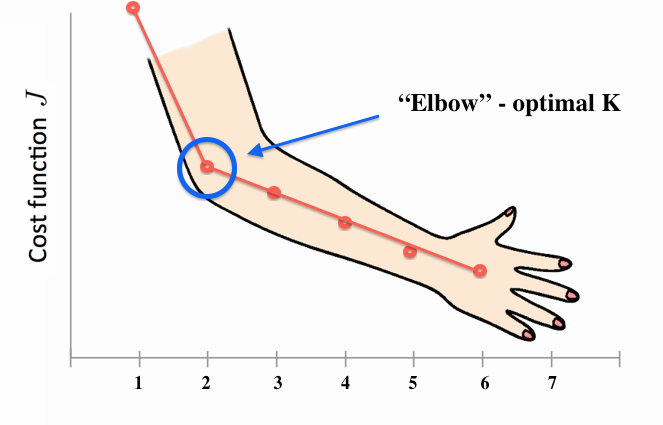
\includegraphics[width=0.6\linewidth]{18.png} 
        \caption{Elbow method illustrated}
        \label{elbow}
      \end{figure}


    \subsubsection{Going from points to images}

      It is easy to interpret all these notions on points. An adaptation if this algorithm to images is possible. The generalization lays in \textbf{features}. In Machine Learning, each training example is described by a set of features. For example a point has two features: \( x \) and \( y \) coordinates. Each training example \( x^{(i)} \) from the vector of examples is a vector itself -- a vector of features. Each feature is a simple number. The Euclidean distance between such training examples is the vector difference. But in order to make features uniform, they should be scaled and normalized. Let the training examples be some houses. Each house is characterized by a a set of features. A feature might be the number of bedrooms (that would be a one-digit number), or the size measured in \( m^2 \), which would be a number tens or hundreds time bigger. Features can have very different numerical values. While computing the distance, some of them might play a much higher role than others which is not the goal. Thus the transformations are performed: \textbf{feature scaling and normalization}.
      Feature scaling has the purpose to bring each \( x^{(i)}_j \) value (where \( x^{(i)}_j \) is the feature \( j \) of example \( x^{(i)} \)) into approximately \( [-1;1] \) range. This is done by simply dividing the current value to the maximal value of one feature across all examples. Feature normalization is the replacement of \( x^{(i)}_j \) with \( x^{(i)}_j - \mu_j \) to make features have approximately zero mean (where \( \mu_j \) is the mean value of feature \( j \) across all examples). 

      One of the most important roles in Machine Learning is played by feature selection. These values are the representative of the training examples. In this thesis, the training examples are the images of objects. The selected features should be good enough to mark the intraclass similarities and interclass differences. This is the list of selected features:
      \begin{enumerate}[topsep=0pt, partopsep=0pt,itemsep=0pt,parsep=1pt]
        \item image width;
        \item image height;
        \item mean red value of the image;
        \item mean blue value of the image;
        \item mean green value of the image;
        \item \( |width - height| \) -- how ``square'' is the image;
        \item image area.
      \end{enumerate}

      % \begin{figure}[hb!]
      %   \centering
      %   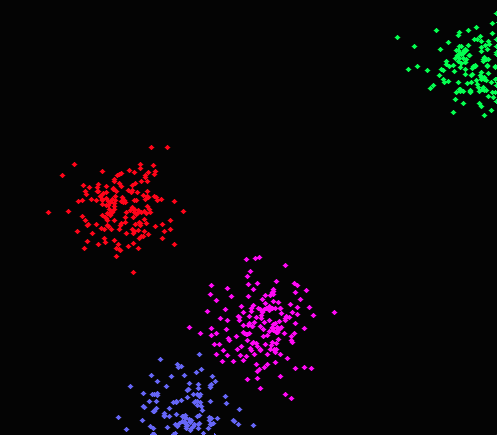
\includegraphics[width=0.525\linewidth]{11.png} 
      %   \caption{The result of OpenCV K-means clustering algorithm}
      %   \label{clusters}
      % \end{figure}

      \begin{figure}[hb!]
        \centering
        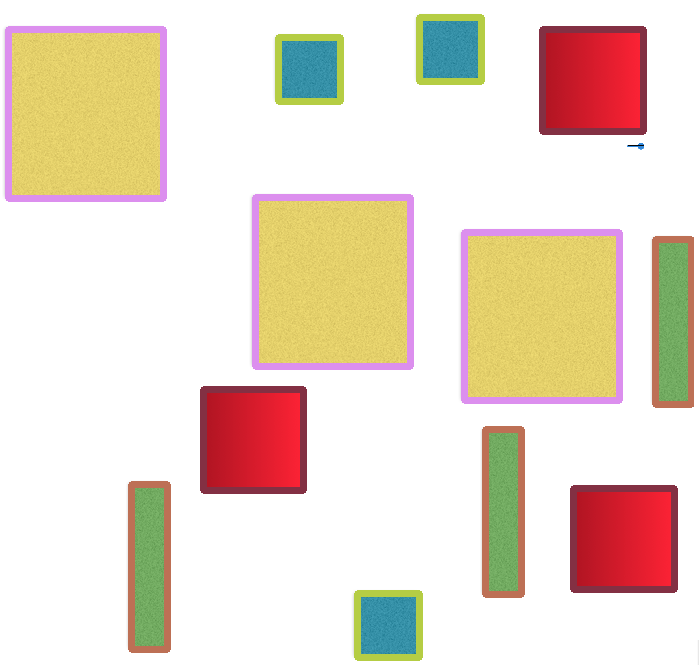
\includegraphics[width=0.35\linewidth]{19.png} 
        \caption{Example of clustering of simple shapes on a test image}
        \label{clusteringEx}
      \end{figure}




\clearpage